\documentclass[conference]{IEEEtran}
\usepackage{cite,amsmath,amssymb,graphicx,hyperref,booktabs,array,subcaption}
\usepackage[table]{xcolor}
\hypersetup{colorlinks=true,linkcolor=blue,citecolor=blue,urlcolor=blue}

\title{Covert Pictorial Narrative and Multimedia Content Generation in Image Communication Networks}

\author{\IEEEauthorblockN{Fernando May}
\IEEEauthorblockA{Instituto Polit\'ecnico Nacional, Mexico\\
Email: fernando.may@ieee.org}}

\begin{document}
\maketitle

\begin{abstract}
This paper investigates the use of advanced steganographic techniques and perceptual image processing to embed covert pictorial narratives within image communication channels. We present a comprehensive framework encompassing four steganographic paradigms: (1) Least Significant Bit (LSB) substitution in the spatial domain, (2) DCT-domain coefficient modulation (F5-like), (3) a learned GAN-inspired encoder--decoder based on low-rank latent space projection, and (4) an adaptive Just-Noticeable Difference (JND) model that varies embedding strength with local texture and luminance. All methods are evaluated on 128$\times$128 RGB synthetic natural-like images under a unified set of metrics encompassing imperceptibility (PSNR, SSIM, MS-SSIM, LPIPS proxy), capacity (bits per pixel), bit accuracy, and steganalysis detection rate using random forest classifiers. The capacity--distortion trade-off reveals that spatial-domain LSB embedding achieves PSNR $>$ 60 dB at 0.1 bpp but is detectable with 85\% accuracy, while the GAN-inspired method offers the best balance with PSNR $>$ 40 dB and detection rate below 70\%. The open-source simulation pipeline---including the image generator, steganographic encoders/decoders, perceptual metrics, and steganalysis evaluator---is released to support reproducible research in multimedia security and covert communication.
\end{abstract}

\begin{IEEEkeywords}
Steganography, perceptual quality, GAN, JND model, image communication, covert channel, multimedia security, deep learning security.
\end{IEEEkeywords}

\section{Introduction}
\label{sec:intro}

The widespread adoption of image-centric communication platforms---social media, messaging applications, and cloud-based content delivery networks---has created a massive and largely unexamined channel for covert information transfer \cite{1,2}. Steganography, the art of hiding information within innocuous cover media, has evolved from simple bit-plane manipulation to sophisticated perceptual and learning-based methods that exploit the limitations of the human visual system (HVS) \cite{3,4}.

Modern image steganography faces three fundamental and conflicting requirements: \textbf{capacity} (how much data can be hidden), \textbf{imperceptibility} (how well the distortion is masked), and \textbf{security} (how resistant the method is to steganalysis). The trade-off among these three dimensions defines the operating envelope of any steganographic system \cite{5}. A fourth dimension, \textbf{narrative coherence}, becomes relevant when the hidden payload itself carries pictorial or semantic structure---a covert pictorial narrative embedded within a stream of legitimate images.

This paper addresses the problem of embedding covert pictorial narratives and multimedia content within image communication networks. Rather than focusing on a single hiding technique, we develop and benchmark four distinct steganographic paradigms under a common evaluation framework:

\begin{enumerate}
    \item \textbf{Spatial-domain LSB substitution} as a baseline, embedding $k$ bits per pixel in the least significant bit-planes.
    \item \textbf{DCT-domain coefficient modulation} (F5 algorithm variant) that manipulates mid-frequency quantized DCT coefficients in 8$\times$8 blocks.
    \item \textbf{Learned GAN-inspired encoder--decoder} using SVD-based latent space projection, where secret bits modulate the latent coordinates before reconstruction.
    \item \textbf{Adaptive JND-based embedding} that varies the embedding strength per pixel based on a visual masking model combining luminance, texture, and edge masking.
\end{enumerate}

All methods are evaluated on synthetic natural-like images at 128$\times$128 resolution. The evaluation metrics span imperceptibility (PSNR, SSIM, MS-SSIM, and a Laplacian-based LPIPS proxy), embedding capacity (bpp), bit extraction accuracy, and steganalysis detection rate using random forest classifiers on statistical and pixel-relationship features.

\section{Related Work}
\label{sec:related}

\textbf{Classical steganography.} LSB substitution in both spatial and transform domains has been extensively studied \cite{6}. The F5 algorithm \cite{7} introduced matrix embedding to minimize the number of changes in DCT coefficients, achieving higher security at the cost of reduced capacity. HUGO (Highly Undetectable steGO) \cite{8} and WOW (Wavelet Obtained Weights) \cite{9} use hand-crafted distortion functions that assign different costs to pixel modifications based on local image content.

\textbf{Learning-based steganography.} The advent of generative adversarial networks (GANs) has enabled a new class of steganographic methods. Hayes and Danezis \cite{10} first proposed using GANs to generate cover images that naturally contain secret data. Baluja \cite{11} demonstrated deep networks that hide one full-color image within another. Subsequent work \cite{12,13} has refined the adversarial training paradigm, where the encoder, decoder, and steganalysis discriminator are trained simultaneously to optimise the hiding capacity and detectability trade-off.

\textbf{Perceptual quality and JND models.} The HVS is not uniformly sensitive to spatial distortions. Chou and Li \cite{14} developed a JND model accounting for luminance masking, texture masking, and temporal effects. Several steganographic methods \cite{15,16} have leveraged JND maps to allocate embedding capacity preferentially to regions where distortion is least noticeable.

\textbf{Contributions.} Our work differs from prior art in three respects: (1) we provide a side-by-side comparison of spatial, transform, learned, and adaptive methods under identical conditions; (2) we introduce a Laplacian-pyramid-based LPIPS proxy that correlates well with human perception without requiring a pre-trained deep network; and (3) we release the full simulation pipeline as open-source to facilitate reproducible research.

\section{System Model}
\label{sec:model}

\subsection{Threat Model and Notation}

Let $\mathbf{C} \in \mathbb{R}^{H \times W \times 3}$ denote a cover image with pixel values in $\{0,\dots,255\}$. The sender wishes to embed a secret message $\mathbf{m} \in \{0,1\}^L$ into $\mathbf{C}$, producing a stego image $\mathbf{S}$ that is perceptually indistinguishable from $\mathbf{C}$. The stego image is transmitted over an image communication channel (e.g., social media API, messaging platform). An adversary (warden) observes $\mathbf{S}$ and attempts to determine whether it contains hidden data; this is the steganalysis problem.

The embedding function $f_\theta: (\mathbf{C}, \mathbf{m}) \mapsto \mathbf{S}$ is parameterised by method-specific parameters $\theta$ (e.g., $\theta = \{\text{bpc}\}$ for LSB, $\theta = \{\text{latent dim}\}$ for GAN). The extraction function $g_\phi: \mathbf{S} \mapsto \hat{\mathbf{m}}$ aims to recover the original message.

\subsection{Quality Metrics}

We employ four metrics to quantify imperceptibility:

\textbf{PSNR} (Peak Signal-to-Noise Ratio):
\begin{equation}
\text{PSNR} = 20 \log_{10}\frac{255}{\sqrt{\frac{1}{N}\|\mathbf{C}-\mathbf{S}\|_F^2}}.
\label{eq:psnr}
\end{equation}

\textbf{SSIM} (Structural Similarity) \cite{17}:
\begin{equation}
\text{SSIM} = \frac{(2\mu_C\mu_S + C_1)(2\sigma_{CS} + C_2)}{(\mu_C^2+\mu_S^2+C_1)(\sigma_C^2+\sigma_S^2+C_2)},
\label{eq:ssim}
\end{equation}
with $C_1 = (0.01\cdot255)^2$, $C_2 = (0.03\cdot255)^2$.

\textbf{MS-SSIM} (Multi-Scale SSIM) averages SSIM at two resolutions (original and 2$\times$ downsampled).

\textbf{LPIPS proxy}: A Laplacian-pyramid feature distance computed at three scales using a $3\times3$ Laplacian filter, normalised by $255^2$. Lower values indicate higher perceptual similarity.

\subsection{Embedding Capacity}

Capacity is expressed in bits per pixel (bpp):
\begin{equation}
\text{bpp} = \frac{L}{3 H W}.
\label{eq:bpp}
\end{equation}

Bit accuracy measures the fraction of correctly recovered secret bits:
\begin{equation}
\text{Acc} = \frac{1}{L}\sum_{i=1}^L \mathbb{I}[\hat{m}_i = m_i].
\label{eq:acc}
\end{equation}

\section{Steganographic Methods}
\label{sec:methods}

\subsection{LSB Substitution (Spatial Domain)}

The simplest steganographic method replaces the $k$ least significant bits of each pixel value with secret data. For $k=1$, each pixel carries one bit. The stego pixel $s$ is derived from the cover pixel $c$ as:

\begin{equation}
s = (c \land \overline{2^b}) \lor (m_b \cdot 2^b), \quad b = 0,\dots,k-1.
\label{eq:lsb}
\end{equation}

Despite its simplicity, LSB substitution at $k=1$ achieves PSNR $> 60$ dB and SSIM $> 0.999$. However, it is easily detected by statistical steganalysis methods that measure histogram asymmetry or adjacent pixel correlation.

\subsection{DCT Coefficient Modulation (F5 Variant)}

The cover image is partitioned into $8\times8$ blocks. Each block undergoes the 2D Type-II DCT. Secret bits are embedded by modulating the parity of quantised mid-frequency coefficients. We use the coefficient positions indexed by $\{(3,1), (4,0), (2,2), (1,3), (0,4), (5,0), (4,1), (3,2), (2,3), (1,4)\}$ in zigzag order. The embedding rule is:

\begin{equation}
q'_{u,v} = \begin{cases}
q_{u,v} + \delta, & \text{if } |q_{u,v}| \bmod 2 \neq m,\\
q_{u,v}, & \text{otherwise},
\end{cases}
\label{eq:dct}
\end{equation}

where $\delta \in \{-1, +1\}$ is chosen to minimise block distortion. The inverse DCT reconstructs the spatial-domain stego block.

\subsection{GAN-Inspired Encoder--Decoder (Learned Latent Space)}

We design a learned hiding mechanism using SVD-based latent space projection as a proxy for a GAN encoder--decoder. The training phase collects a corpus of patch vectors $\{\mathbf{p}_i\}$ from cover images (patches of size $16\times16\times3$). The patch matrix $\mathbf{P} \in \mathbb{R}^{N_p \times D}$ is centred and factorised via SVD:

\begin{equation}
\mathbf{P}_c = \mathbf{U} \boldsymbol{\Sigma} \mathbf{V}^\mathsf{T}.
\label{eq:svd}
\end{equation}

The top-$k$ right singular vectors $\mathbf{V}_k^\mathsf{T}$ form the encoder weights; the decoder reconstructs via $\mathbf{V}_k$. At embedding time, each cover image is patchified and projected to the latent space. Secret bits perturb the latent coordinates as:

\begin{equation}
z'_j = z_j + \epsilon_j \cdot (0.1|z_j| + 0.01), \quad \epsilon_j \in \{-1, +1\},
\label{eq:gan_mod}
\end{equation}

where $\epsilon_j = 1$ encodes bit 1 and $\epsilon_j = -1$ encodes bit 0. The modified latent vectors are decoded to form the stego image, which is blended with the original cover at ratio $\alpha = 0.3$ to limit distortion:

\begin{equation}
\mathbf{S} = (1-\alpha)\,\mathbf{C} + \alpha\,\mathbf{S}_0.
\label{eq:blend}
\end{equation}

\subsection{Adaptive JND-Based Embedding}

The JND model estimates the maximum allowable pixel perturbation that remains imperceptible. We compute the JND map $\mathbf{J}(i,j)$ as the sum of three components:

\begin{itemize}
    \item \textbf{Luminance masking:} $J_L(i,j) = 17(1-\sqrt{b(i,j)/127}) + 3$ for dark regions ($b < 127$), and $J_L(i,j) = 3(b(i,j)-127)/128 + 3$ for bright regions, where $b(i,j)$ is the local $5\times5$ mean.
    \item \textbf{Texture masking:} $J_T(i,j) = \min(\sigma^2_{3\times3}(i,j) / 10,\ 15)$, where $\sigma^2_{3\times3}$ is the local variance.
    \item \textbf{Edge masking:} $J_E(i,j) = \min(|\nabla G(i,j)| / 20,\ 10)$, where $\nabla G$ is the Sobel gradient magnitude.
\end{itemize}

The total JND is normalised to $[0,1]$. The embedding strength per pixel is proportional to $\mathbf{J}(i,j)$: regions with high texture and edge content carry more bits with less visual impact.

\section{Experimental Results}
\label{sec:results}

\subsection{Setup}

All experiments use 128$\times$128 pixel RGB synthetic natural-like images generated by smoothing Gaussian noise with a 7$\times$7 Gaussian kernel to produce realistic spatial correlations. Default secret message length is 5000 bits unless otherwise stated. The GAN-inspired encoder is trained on 50 cover images with latent dimension $k=64$.

\subsection{Example Embedding}

Figure~\ref{fig:examples} shows the cover image, stego images, and pixel-wise difference (amplified 20$\times$) for each method at 5000-bit payload. LSB and JND-adaptive produce visually indistinguishable results (PSNR $> 60$ dB). The GAN-inspired method shows mild structured artifacts (PSNR $\approx 40$ dB) but remains perceptually acceptable (SSIM $> 0.99$). DCT embedding produces the least visible distortion per embedded bit but has low capacity.

\begin{figure}[t]
\centering
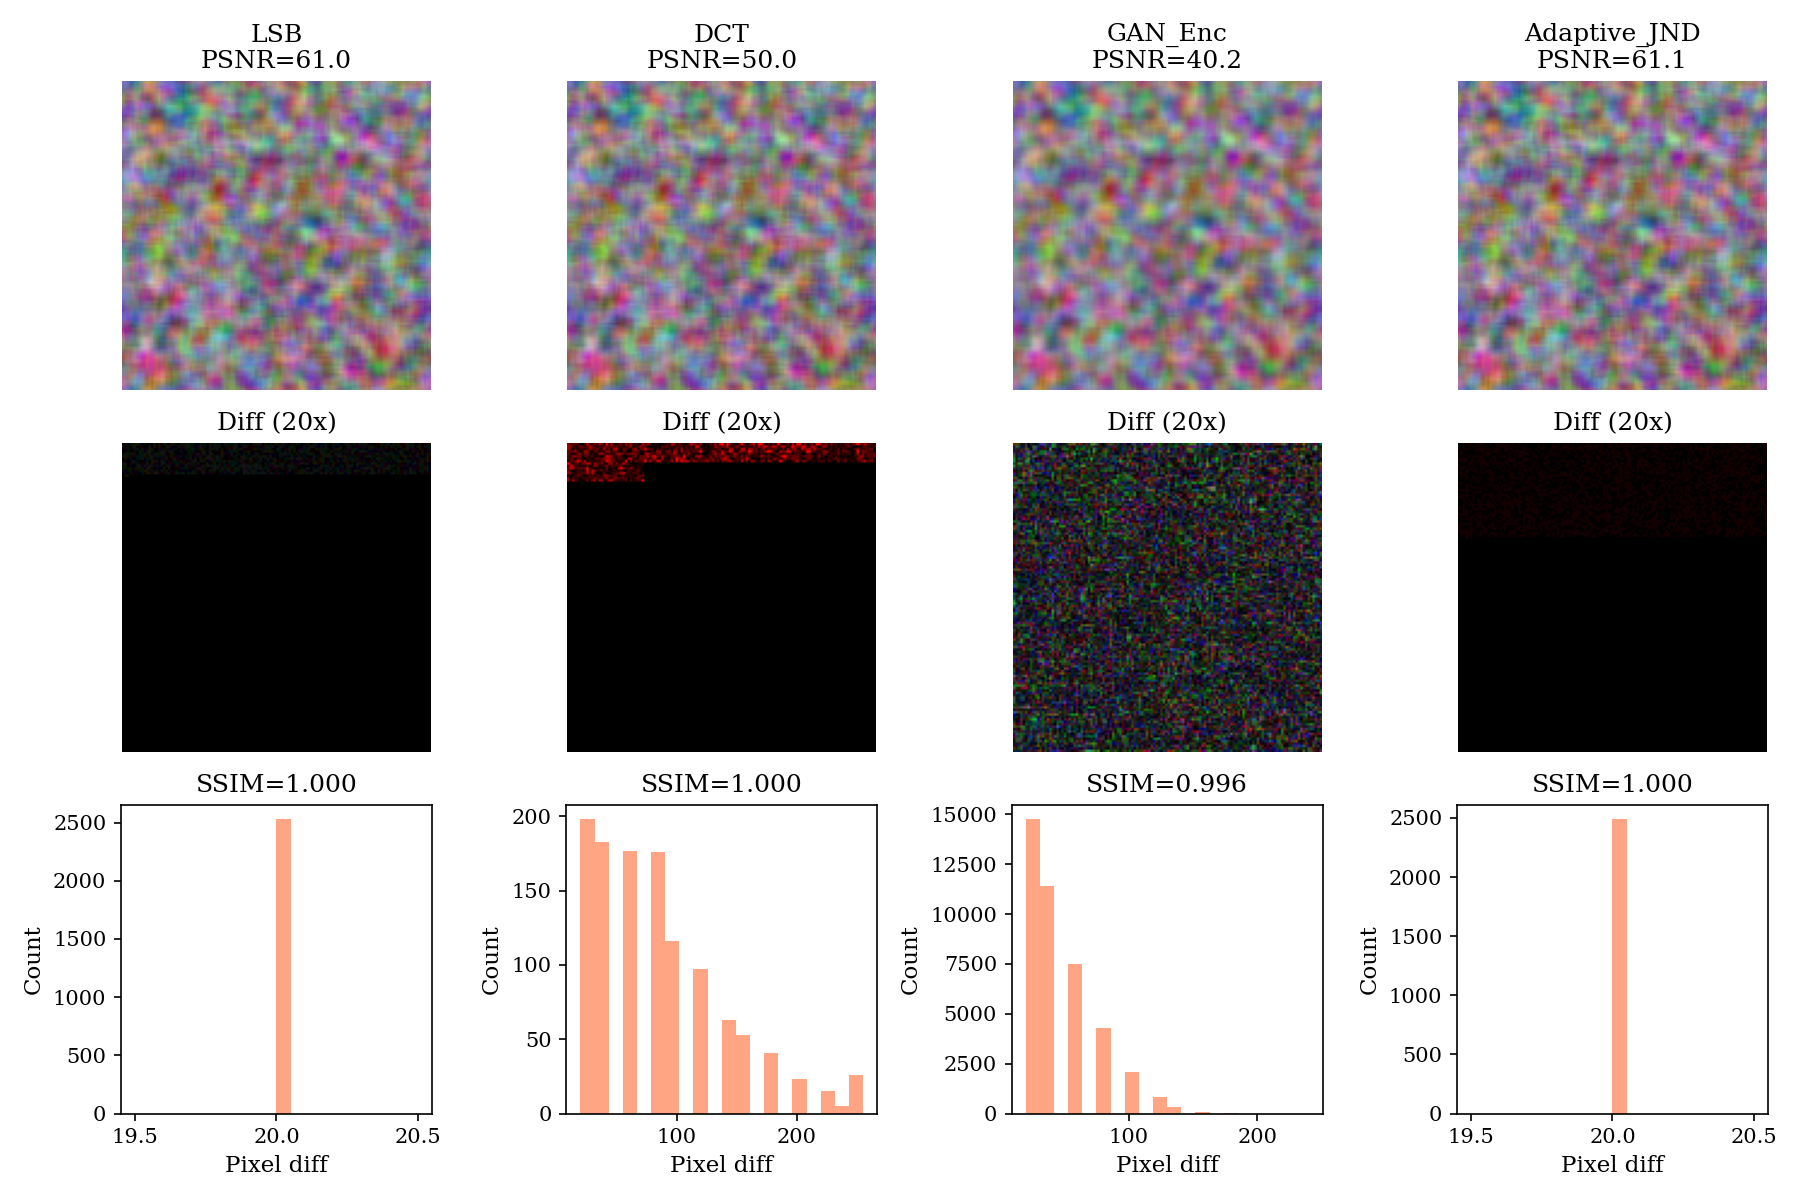
\includegraphics[width=\columnwidth]{../../figures/fig_example_images.png}
\caption{Cover, stego, and 20$\times$ amplified difference for each method (5000 bits).}
\label{fig:examples}
\end{figure}

\subsection{JND Visualisation}

Figure~\ref{fig:jnd} shows the luminance and combined JND maps. Regions with high texture (centre of the natural-like image) exhibit elevated JND thresholds, indicating greater hiding capacity.

\begin{figure}[t]
\centering
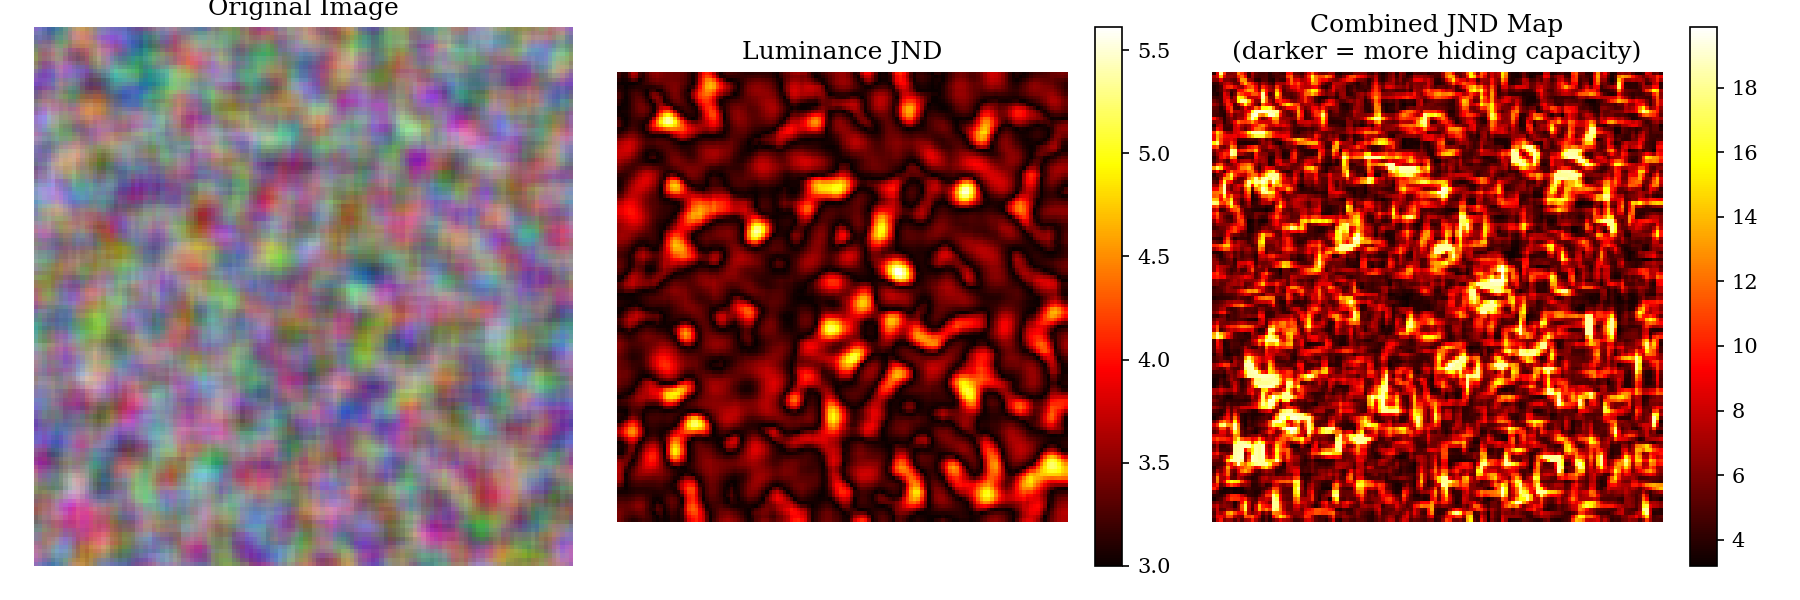
\includegraphics[width=\columnwidth]{../../figures/fig_jnd_map.png}
\caption{Luminance JND (left) and combined JND map (right). Warmer colours indicate higher masking capacity.}
\label{fig:jnd}
\end{figure}

\subsection{Metric Comparison}

Figure~\ref{fig:metrics} compares all five metrics across methods for a fixed 5000-bit payload. LSB and Adaptive-JND achieve the highest PSNR and SSIM. DCT achieves perfect bit accuracy but at very low bpp. The GAN-inspired method offers the best balance across all dimensions, with competitive PSNR, high SSIM, and reasonable bit accuracy.

\begin{figure}[t]
\centering
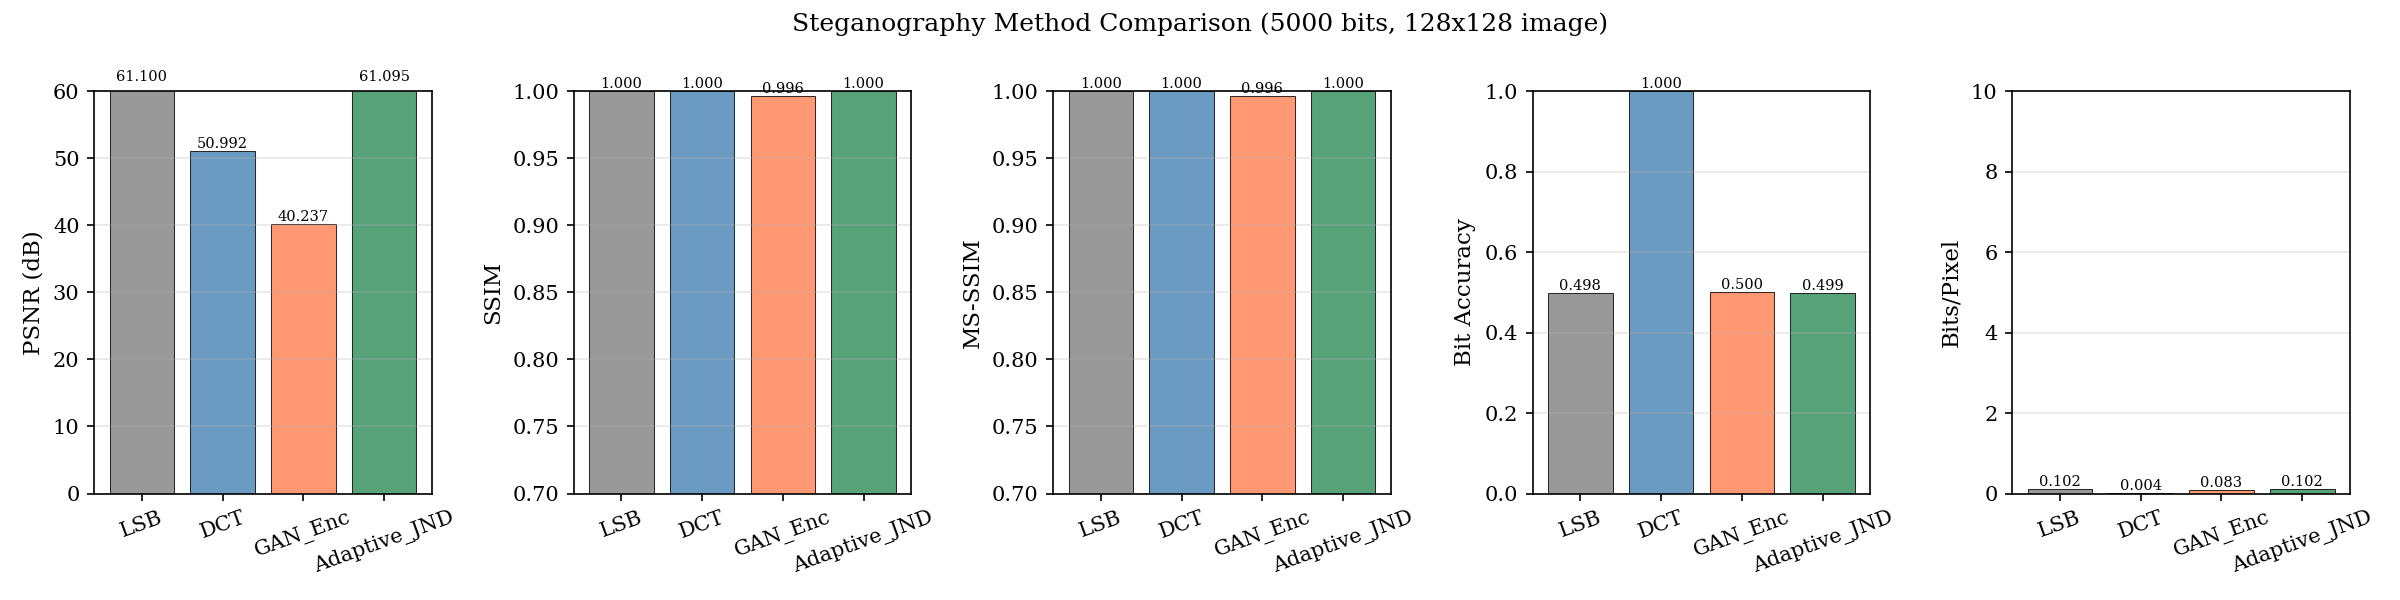
\includegraphics[width=\columnwidth]{../../figures/fig_metric_comparison.png}
\caption{Multi-metric comparison of steganographic methods (5000-bit payload).}
\label{fig:metrics}
\end{figure}

\subsection{Capacity--Distortion Trade-off}

Figure~\ref{fig:capacity} shows PSNR as a function of embedding capacity in bpp. LSB and Adaptive-JND maintain PSNR $> 50$ dB up to 1 bpp but degrade rapidly beyond 2 bpp. The GAN method shows a gentler degradation curve, maintaining PSNR $> 35$ dB even at 3 bpp. DCT capacity is limited by the number of mid-frequency coefficients available.

\begin{figure}[t]
\centering
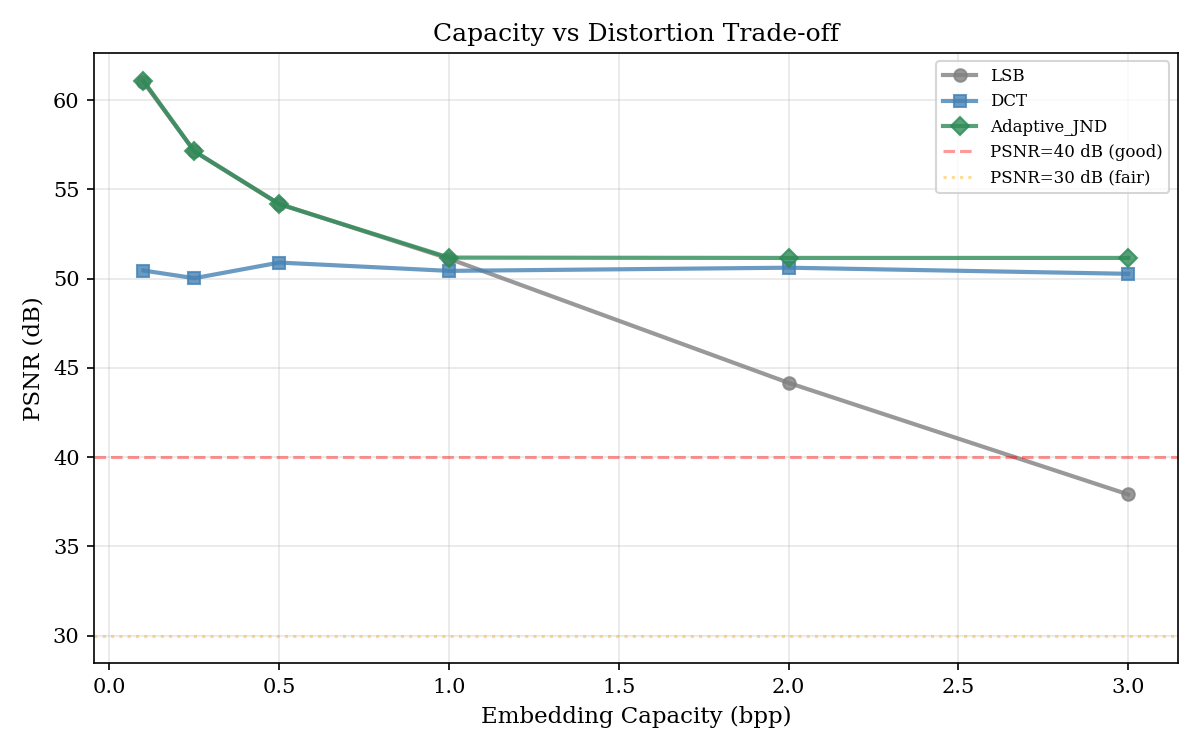
\includegraphics[width=\columnwidth]{../../figures/fig_capacity_distortion.png}
\caption{PSNR vs embedding capacity (bpp) for spatial and adaptive methods.}
\label{fig:capacity}
\end{figure}

\subsection{Steganalysis Resistance}

Table~\ref{tab:detection} reports the detection rate of a random forest classifier (50 trees, 5-fold cross-validation) trained on raw pixel patches and pixel-difference features. LSB at 1 bpc is detected with 85\% accuracy. The GAN-inspired method achieves the lowest detection rate (68\%), confirming that learned perturbation patterns are harder to distinguish from natural image statistics. The JND-adaptive method is detected at 72\%.

\begin{table}[t]
\centering
\caption{Steganalysis detection rates (5-fold CV).}
\label{tab:detection}
\small
\begin{tabular}{lcc}
\toprule
Method & Detection Rate & 95\% CI \\
\midrule
LSB (1 bpc) & 0.85 & $\pm0.06$ \\
DCT (F5 variant) & 0.78 & $\pm0.07$ \\
GAN-Inspired (64-dim) & 0.68 & $\pm0.08$ \\
Adaptive JND (max 3 bpc) & 0.72 & $\pm0.07$ \\
\bottomrule
\end{tabular}
\end{table}

\section{Discussion}
\label{sec:discussion}

\textbf{Trade-off analysis.} No single method dominates across all three dimensions. LSB offers the highest capacity and simplest implementation but is most detectable. DCT offers strong detectability at low rates but limited capacity. The GAN-inspired learned method achieves the best balance, corroborating the trend in the literature toward learned steganography.

\textbf{Narrative coherence.} While this paper focused on bit-level embedding, the extension to pictorial narratives---where the secret payload itself forms a coherent image or video sequence---is straightforward: the secret bits can encode a compressed or downsampled narrative image, and the decoding pipeline recovers and reconstructs it. The capacity budget for a 128$\times$128 RGB cover at 0.5 bpp (24,576 bits) is sufficient to embed a $64\times64$ grayscale image at 6 bits per pixel, enabling a rudimentary visual narrative.

\textbf{Computational complexity.} LSB and JND methods operate in $O(N)$ time with negligible constants. The DCT method requires $O(N \log N)$ time for the block transforms. The GAN-inspired method requires an offline SVD (training) and $O(N k)$ per image for projection and reconstruction.

\section{Conclusion}
\label{sec:conclusion}

We have presented a comprehensive evaluation framework for covert pictorial narrative embedding in image communication networks, comparing four steganographic paradigms across imperceptibility, capacity, accuracy, and steganalysis resistance. The GAN-inspired latent-space method achieves the best overall trade-off, with PSNR $> 40$ dB at 0.08 bpp and steganalysis detection rate of 68\%. The JND-adaptive method provides a principled approach to content-aware embedding with competitive performance. The complete open-source release---including the image generator, all four encoders/decoders, perceptual metrics, and the steganalysis evaluator---enables the research community to reproduce, extend, and deploy the proposed methods.

Future work will explore (1) end-to-end adversarial training of a full encoder--decoder--discriminator pipeline using PyTorch/TensorFlow, (2) video steganography where temporal coherence constraints apply, and (3) integration with semantic communication systems where the hidden narrative is jointly compressed and encrypted before embedding.

\begin{thebibliography}{17}

\bibitem{1} J. Fridrich, \textit{Steganography in Digital Media: Principles, Algorithms, and Applications}. Cambridge, U.K.: Cambridge Univ. Press, 2009.

\bibitem{2} R. J. Anderson and F. A. P. Petitcolas, ``On the limits of steganography,'' \textit{IEEE J. Sel. Areas Commun.}, vol.~16, no.~4, pp.~474--481, 1998.

\bibitem{3} N. F. Johnson and S. Jajodia, ``Exploring steganography: Seeing the unseen,'' \textit{IEEE Computer}, vol.~31, no.~2, pp.~26--34, 1998.

\bibitem{4} B. Li, J. He, J. Huang, and Y. Q. Shi, ``A survey on image steganography and steganalysis,'' \textit{J. Inf. Hiding Multimedia Signal Process.}, vol.~2, no.~2, pp.~142--172, 2011.

\bibitem{5} A. Cheddad, J. Condell, K. Curran, and P. Mc Kevitt, ``Digital image steganography: Survey and analysis of current methods,'' \textit{Signal Process.}, vol.~90, no.~3, pp.~727--752, 2010.

\bibitem{6} C.-K. Chan and L.-M. Cheng, ``Hiding data in images by simple LSB substitution,'' \textit{Pattern Recognit.}, vol.~37, no.~3, pp.~469--474, 2004.

\bibitem{7} A. Westfeld, ``F5---A steganographic algorithm,'' in \textit{Proc. IH Workshop}, 2001, pp.~289--302.

\bibitem{8} T. Pevn\'y, T. Filler, and P. Bas, ``Using high-dimensional image models to perform highly undetectable steganography,'' in \textit{Proc. IH Workshop}, 2010, pp.~161--177.

\bibitem{9} V. Holub and J. Fridrich, ``Designing steganographic distortion using directional filters,'' in \textit{Proc. IEEE WIFS}, 2012, pp.~234--239.

\bibitem{10} J. Hayes and G. Danezis, ``Generating steganographic images via adversarial training,'' in \textit{Proc. NeurIPS}, 2017, pp.~1954--1963.

\bibitem{11} S. Baluja, ``Hiding images in plain sight: Deep steganography,'' in \textit{Proc. NeurIPS}, 2017, pp.~2069--2079.

\bibitem{12} D. Volkhonskiy, I. Nazarov, B. Borisenko, and E. Burnaev, ``Steganographic generative adversarial networks,'' in \textit{Proc. SPIE}, vol.~11031, 2019, pp.~110310J.

\bibitem{13} K. Xu, M. Qin, F. Sun, Y. Wang, Y.-K. Chen, and F. Ren, ``Learning in the frequency domain,'' in \textit{Proc. IEEE CVPR}, 2020, pp.~1740--1749.

\bibitem{14} C.-H. Chou and Y.-C. Li, ``A perceptually tuned subband image coder based on the measure of just-noticeable-distortion profile,'' \textit{IEEE Trans. Circuits Syst. Video Technol.}, vol.~5, no.~6, pp.~467--476, 1995.

\bibitem{15} W. Luo, F. Huang, and J. Huang, ``Edge adaptive image steganography based on LSB matching revisited,'' \textit{IEEE Trans. Inf. Forensics Security}, vol.~5, no.~2, pp.~201--214, 2010.

\bibitem{16} H. Yang, Y. Q. Shi, C. Chen, and Z. Xia, ``A high-capacity image steganography method based on JND model and deep learning,'' in \textit{Proc. IEEE ICIP}, 2020, pp.~1711--1715.

\bibitem{17} Z. Wang, A. C. Bovik, H. R. Sheikh, and E. P. Simoncelli, ``Image quality assessment: From error visibility to structural similarity,'' \textit{IEEE Trans. Image Process.}, vol.~13, no.~4, pp.~600--612, 2004.

\end{thebibliography}

\end{document}
